\documentclass{ssiBio}
\usepackage{siunitx}
\usepackage{verbatim}
\title{Polyamine Environment Experiment} % CHANGE THIS
\author{Written by \textbf{Kaitlin Hsu}}
\date{\textbf{Written:} January 24, 2019 \,\textbf{Performed:} January 26, 2019 \,\textbf{Printed:} \today{}}

\begin{document}

\maketitle
\section{Procedure Purpose} % CHANGE THIS
Aim to improve the efficiency of the backspace method by seeing if a polyamine environment affects Exoncuclease T cleavage in DNA strands.
\section{Overview} % CHANGE THIS
\begin{comment}
In order to conduct DNA synthesis using water-soluble and non-toxic materials, a method using a pair of enzymes to extend and shorten a pre-existing template strand has been devised and termed the 'backspace' method. This technique involves three steps:
\begin{enumerate}
\item{Elongating an existing single-stranded DNA strand with an arbitrary tail of one nucleotide using Terminal Deoxynucleotidyl Transferase (TdT).}
\item{Adding a complementary strand that matches the 3' end of the original starting sequence, as well as one or two of the added nucleotides.}
\item{Introducing Exonuclease T, which will cleave the 3' region of the elongated starting strand, effectively cleaving excess nucleotides that are not to be added to the final product. \cite{zuo_deutscher_1999}}
\end{enumerate}
\end{comment}
This experiment is intended to determine how a polyamine environment affect Exonuclease T activity. We are introducing this environment through the addition of spermine, spermidine, and putrescine.

At physiological levels, the presence of these polyamines causes DNA to condense through site-specific, structural, and electrostatic interactions. The increased stability may protect against overcutting by Exonuclease T.This protocol builds on previous experiments undertaken using Exonuclease T. \cite{tomusiak} \cite{uttmark} \cite{ringach} \cite{tomusiak2}
% Safety First! ALSO, % CHANGE THIS
\section{Safety Information}
\begin{safety}
\begin{enumerate}
\SYBRGOLD{}
\item{When diluting the polyamines, work in fume hood when possible, especially when you're doing those dilutions from really concentrated stock.}
\item{Working in a communal lab space is dangerous. Do not assume your fellow workers cleaned up sufficiently.}
\end{enumerate}
\end{safety}

\section{Materials}
\begin{itemize}
\item{``BS\_Start\_pos5" Oligonucleotide (Sequence:  5'-AGTTACCATGACCGTGTGCGTTTTT-3')}
%\item{``BS\_Start\_pos5A" Oligonucleotide (Sequence:  5'-AGTTACCATGACCGTGTGCGAAAAA-3')}
%\item{``BS\_Start\_pos5C" Oligonucleotide (Sequence:  5'-AGTTACCATGACCGTGTGCGCCCCC-3')}
%\item{``BS\_Start\_pos\_3" Oligonucleotide (Sequence:  5'-AGTTACCATGACCGTGTGCGTTT-3')}
\item{``BS\_Start\_pos" Oligonucleotide (Sequence:  5'-AGTTACCATGACCGTGTGCGT-3')}
\item{``BS\_Start" Oligonucleotide (Sequence:  5'-AGTTACCATGACCGTGTGCG-3')}
\item{``BS\_Comp\_6" Oligonucleotide (Sequence:  5'-AACGCA-3')}
\item{Spermine (1g)}
\item{Spermidine (1g)}
\item{Putrescine (1g)}
%\item{``BS\_thio\_6\_fluoro\_6" Oligonucleotide (Sequence:  5'-A*A*C*G*C*A-3'), with all 2' fluorine-modified bases}
%\item{``BS\_fluoro\_6" Oligonucleotide (Sequence:  5'-AACGCA-3'), with all 2' fluorine-modified bases}
%\item{``BS\_Comp\_6\_3ext" Oligonucleotide (Sequence:  5'-AAACGCA-3')}
%\item{``BS\_Comp\_7" Oligonucleotide (Sequence:  5'-AACGCAC-3')}
%\item{``BS\_Comp\_8" Oligonucleotide (Sequence:  5'-AACGCACA-3')}
%\item{``BS\_Comp\_9" Oligonucleotide (Sequence:  5'-AACGCACAC-3')}
%\item{``BS\_Comp\_10\_2" Oligonucleotide (Sequence:  5'-AACGCACACG-3')}
%\item{``BS\_Comp\_6F" Oligonucleotide (Sequence:  5'-CCCGCA-3')}
%\item{``BS\_Comp\_6G" Oligonucleotide (Sequence:  5'-GGCGCA-3')}
\item{Exonuclease T (5 U/\uL{})}
\item{SYBR Gold (10,000X)}
\item{NEBuffer 4 (10X)}
\item{TBE Buffer (1X)}
\item{Gel Loading Buffer II (2X)}
\item{Two Novex TBE Gels (20\%)}
\item{IDT 10/60 Ladder}
\item{RNAse Free Water}
\item{RNAse Free PCR tubes}
\item{RNAse Free pipette tips}
\item{Two thermocyclers}
\end{itemize}
% Now for the _good_ stuff
\section{Dilutions}
\begin{enumerate}
\item{Dilute each of the oligonucleotides listed in 'Materials' to a 100uM liquid stock in RNAse free water. Thoroughly vortex and store modified oligos at -20C after use.}
\item{Dilute each of the complementary oligonucleotides listed (except and BS\_Comp\_6) to 10uM working stock by putting 5 uL of the 100 uM stock in 45 uL RNAse free water.}
\item{Dilute BS\_Comp\_6 to 10uM working stock by putting 15 uL of the 100 uM stock in 135 uL RNAse free water.}

\item{Dilute 1g of spermine to 5M working stock by adding .574 mL of RNAse free water into the bottle.}
\item{Dilute 5M spermine to 5mM working stock by adding 1\uL{} of the 5M stock to 999\uL{} of RNAse free water.}
\item{Dilute 5mM spermine to 100uM working stock by adding 10 \uL{} of 5mM stock to 490\uL{} of RNAse free water.}
\item{Dilute 100uM spermine to 50uM working stock by adding 50 \uL{} of 100uM stock to 50\uL{} of RNAse free water.}
\item{Dilute 100uM spermine to 10uM working stock by adding 10 \uL{} of 100uM stock to 90\uL{} of RNAse free water.}

\item{Dilute 1g of spermidine to 5M working stock by adding 1.38 mL of RNAse free water into the bottle.}
\item{Dilute 5M spermidine to 5mM working stock by adding 1\uL{} of the 5M stock to 999\uL{} of RNAse free water.}
\item{Dilute 5mM spermidine to 100uM working stock by adding 10 \uL{} of 5mM stock to 490\uL{} of RNAse free water.}
\item{Dilute 100uM spermidine to 50uM working stock by adding 50 \uL{} of 100uM stock to 50\uL{} of RNAse free water.}
\item{Dilute 100uM spermidine to 10uM working stock by adding 10 \uL{} of 100uM stock to 90\uL{} of RNAse free water.}

\item{Dilute 1g of putrescine to 5M working stock by adding 2.27 mL of RNAse free water into the bottle.}
\item{Dilute 5M putrescine to 5mM working stock by adding 1\uL{} of the 5M stock to 999\uL{} of RNAse free water.}
\item{Dilute 5mM putrescine to 100uM working stock by adding 10 \uL{} of 5mM stock to 490\uL{} of RNAse free water.}
\item{Dilute 100uM putrescine to 50uM working stock by adding 50 \uL{} of 100uM stock to 50\uL{} of RNAse free water.}
\item{Dilute 100uM putrescine to 10uM working stock by adding 10 \uL{} of 100uM stock to 90\uL{} of RNAse free water.}

%\item{Create a 2.22 fold dilution of ``BS\_Comp\_6" by adding 13.5\uL{} of ``BS\_Comp\_6" to 16.5\uL{} nuclease free water in a tube labeled "BS6Dil".}

\end{enumerate}

\section{Procedure}% CHANGE THIS
\subsection{Sample Explanations}
Consult the following list for a functional explanation of each sample tube:
\begin{enumerate}

\item{S0.5, S2.5, S12.5 refer to samples that will have 0.5, 2.5, and 12.5 micromolar concentrations, respectively, of spermine to test whether the presence of that polyamine will increase the efficiency of Exonuclease T halting at the correct position.}

\item{SD0.5, SD2.5, SD12.5 refer to samples that will have .5, 2.5, and 12.5 micromolar concentrations, respectively, of spermidine to test whether the presence of that polyamine will increase the efficiency of Exonuclease T halting at the correct position.}

\item{P0.5, P2.5, P12.5 refer to samples that will have 0.5, 2.5, and 12.5 micromolar concentrations, respectively, of putrescine to test whether the presence of that polyamine will increase the efficiency of Exonuclease T halting at the correct position.}

\item{Replicates will be prepared for all the same solutions. The tubes will be labeled exactly the same but with an "R" at the end.}

%\item{TF will have a complementary strand modified with all phosphorothioate bonds and all 2'-Fluorine bases, to increase nuclease resistance and increase binding efficiency by combining phosphorothioate and fluorine effects.}
%\item{F will have a complementary strand modified with all 2'-fluorine bonds to control for the effect of only fluorine-modified bases (some nuclease resistance and some increased binding affinity).}
\item{P refers to a positive control (the 21-bp starting DNA strand) bound to a DNA complementary strand (BS\_Comp\_6), N refers to a negative control (the 20-bp unextended DNA strand) bound to a complementary strand (BS\_Comp\_6). }
\item{The D control (for DNA) contains BS\_Start\_pos5, BS\_Comp\_6, and ExoNuclease T with no polyamines.}
\item{The E control contains only the extended starting strand, ``BS\_Start\_pos5," as a length comparison and to ensure there is no manufacturer defect with the starting strand.} %or ``BS\_Start\_pos\_3".}

%\item{N100 refers to a lane containing 100\% (molar ratio) of a 20-base pair DNA strand for length comparison.}
%20-100 percentage of 21-mer, 40 has 80% by mass of 25-mer, 21-mer + RNA, 21-mer+LNA, 20-mer 100%
\end{enumerate}

\subsection{Quantitative Control Preparation}
\begin{enumerate}
%\item{Clean work surface, gloves, and all pipettes with RNAse inhibitor spray.}
\item{Label PCR Tubes according to Table 1.}

\begin{table}[ht]
\begin{tabular}{|l|l|l|l|l|l|}
\hline
                      & \multicolumn{3}{l|}{PCR Tube Labeling} \\ \hline
Spermine Samples      & S0.5   & S2.5   & S12.5         \\ \hline
Spermidine Samples    & SD0.5  & SD2.5  & SD12.5       \\ \hline
Putrescine Samples    & P0.5   & P2.5   & P12.5        \\ \hline
Positive Controls     & P      & P      &                     \\ \hline
Negative Controls     & N      & D      &                     \\ \hline
Quantitative Controls & E      &        &                \\ \hline
\end{tabular}
\end{table}
\item{Into tube `E', add 2.09 \uL{} of 10 uM `BS\_Start\_pos5' oligonucleotide and 22.91 \uL{} of water. Vortex.}

\end{enumerate}

%\stopPoint{}

\subsection{Complementary Strand Annealing}
\begin{enumerate}
\item{Pipette 2.92\uL{} nuclease-free water into PCR Tubes S0.5, S2.5, SD0.5, SD2.5, P0.5, P2.5.}
\item{Pipette 1.42\uL{} nuclease-free water into PCR Tubes S12.5, SD12.5, P12.5.}
\item{Pipette 3.92 \uL{} nuclease-free water into PCR Tube D.}
\item{Pipette 5.52 \uL{} nuclease-free water into PCR Tubes P and N.}

\item{Pipette 1\uL{} of 10uM spermine into PCR Tube S0.5.}
\item{Pipette 1\uL{} of 10uM spermidine into PCR Tube SD0.5.}
\item{Pipette 1\uL{} of 10uM putrescine into PCR Tube P0.5.}

\item{Pipette 1\uL{} of 50uM spermine into PCR Tube S2.5.}
\item{Pipette 1\uL{} of 50uM spermidine into PCR Tube SD2.5.}
\item{Pipette 1\uL{} of 50uM putrescine into PCR Tube P2.5.}

\item{Pipette 2.5\uL{} of 100uM spermine into PCR Tube S12.5.}
\item{Pipette 2.5\uL{} of 100uM spermidine into PCR Tube SD12.5.}
\item{Pipette 2.5\uL{} of 100uM putrescine into PCR Tube P12.5.}

\item{Pipette in 2\uL{} of 10X NEBuffer 4 into PCR Tubes P, N, D, S0.5, S2.5, S12.5, SD0.5, SD2.5, SD12.5, P0.5, P2.5, P12.5.}
\item{Pipette in 3.16\uL{} of 10$\mu$M `BS\_Start\_pos5' 25mer working stock into PCR Tubes D, S0.5, S2.5, S12.5, SD0.5, SD2.5, SD12.5, P0.5, P2.5, and P12.5.}
\item{Pipette in 3.16\uL{} of 10$\mu$M `BS\_Start\_pos' 21mer working stock into PCR tube P.}
\item{Pipette in 3.16\uL{} of 10$\mu$M `BS\_Start' 20mer working stock into PCR tube N.}
\item{Pipette in 9.32\uL{} of 10$\mu$M of ``BS\_Comp\_6" working stock into PCR tubes P, N, D, S0.5, S2.5, S12.5, SD0.5, SD2.5, SD12.5, P0.5, P2.5, and P12.5.}
\item{Put all test samples and positive and negative controls into the thermocycler.}
\item{Set thermocycler to hold at 94◦C for two minutes, then lower the temperature to 5◦C forever at a rate of 0.5\C{} per second.}
\end{enumerate}

\subsection{Exonuclease T Incubation}

%Do the following twice to create replicates. Follow the same protocol for the replicate tubes (which are followed by an R) as for the original sample tubes.
\begin{enumerate}
%Goal: 20uL reactions
\item{Keeping the samples \textbf{in the thermocycler}, pipette 1.6 \uL{} Exonuclease T into each test sample tube (S0.5, S2.5, S12.5, SD0.5, SD2.5, SD12.5, P0.5, P2.5, P12.5) and D.}
\item{Incubate for 1 hour at 5\C{}.}
%\item{Prepare an extra thermocycler set to 95\C{}.}
\item{Pipette 5\uL{} of RNAse-free 500 mM EDTA into each test sample, positive control, and negative control tube.}
%\item{Heat inactivate by transferring all PCR tubes quickly to the 95\C{} thermocycler. Allow incubation for fifteen minutes.}
\end{enumerate}


\stopPoint{}

\subsection{XCell Surelock Setup and Pre-Run}
\begin{enumerate}
\item{Remove two 20\% polyacrylamide gels from pouches and rinse with deionized water.}
\item{Peel off tape on bottom of 20\% polyacrylamide gels and remove combs.}
\item{Lower the Buffer Core (the piece that holds the gels) into the Lower Buffer Chamber so that the negative electrode fits into the opening in the gold plate.}
\item{Insert the Gel Tension Wedge into the XCell Surelock behind the buffer core. Make sure it is in its `unlocked' position, which allows the wedge to slip into the unit.}
\item{Insert gel cassettes into the lower buffer chamber. The shorter ``well" side of the cassette faces into the buffer core. The slot on the back must face outward. If only one gel is being run, insert a buffer dam in the place of a gel cassette.}
\item{Pull forward on the Gel Tension Lever toward the buffer core until the gel cassettes are snug against the buffer core. This puts it in the 'locked' position.}
\item{Fill the Upper Buffer Chamber (between the gels) with 1x TBE running buffer. Ensure it is not leaking.}
\item{Fill the Lower Buffer Chamber completely with running buffer by pouring 1x TBE next to the Gel Tension Wedge.}
\item{Wash each gel well with 12 \uL{} running buffer.}
\item{Place the gel cover on the apparatus in the correct orientation. Connect the electrodes to the power source, and pre-run the gel for 30 minutes at 200V.}
\end{enumerate}

\subsection{Sample Preparation for Gel Running}
%\begin{enumerate}
\begin{figure}[ht] %This is a figure, in this case, a well plate
\begin{center}
\begin{tabular}{|l|l|}
\hline
Well number    & Sample \\ \hline
1                                  & *misloaded* 10/60 Ladder \\ \hline
2                                  & *misloaded* N \\ \hline
3                                  & S0.5 \\ \hline
4                                  & S2.5 \\ \hline
5                                  & S12.5 \\ \hline
6                                  & P \\ \hline
7                                  & SD0.5 \\ \hline
8								   & SD2.5 \\ \hline
9                                  & SD12.5 \\ \hline
10                                 & D \\ \hline
11								   & P0.5 \\ \hline
12                                 & P2.5 \\ \hline
13								   & P12.5 \\ \hline
14                                 & P  \\ \hline
15                                 & *not loaded* E  \\ \hline

\end{tabular}
\label{tab:Gel 1 Layout} %Label your stuff, this is for referencing in the future
\caption{Gel 1} %Caption!
\end{center}
\end{figure}

\begin{figure}[ht] %This is a figure, in this case, a well plate
\begin{center}
\begin{tabular}{|l|l|}
\hline
Well number    & Sample \\ \hline
1                                  & 10/60 Ladder   \\ \hline
2                                  & N   \\ \hline
3                                  & S0.5R \\ \hline
4                                  & S2.5R \\ \hline
5                                  & S12.5R \\ \hline
6                                  & P \\ \hline
7                                  & DR \\ \hline
8                                  & SD0.5R \\ \hline
9								   & SD2.5R \\ \hline
10                                 & SD12.5R \\ \hline
11                                 & P  \\ \hline
12                                 & E  \\ \hline
13								   & P0.5R \\ \hline
14                                 & P2.5R \\ \hline
15								   & P12.5R \\ \hline


\end{tabular}
\label{tab:Gel 2 Layout} %Label your stuff, this is for referencing in the future
\caption{Gel 2} %Caption!
\end{center}
\end{figure}

%\item{Centrifuge each tube for a short period of time. If no fitting centrifuge is present, skip this step.}
%\item{Shortly before inserting the samples into the gel wells, heat for 95\C{} for five minutes. Ensure loading of samples while they are still hot.}
%\end{enumerate}
\subsection{Gel Loading and Running}
\begin{enumerate}
\item{Obtain a sizable piece of parafilm. Pipette 5 \uL{} of 2x Gel Loading Buffer II in two 5 x 3 grids of droplets, and label each droplet with the corresponding sample.}
%\item {For well 1 of Gel 1 and Gel 2, load 6.5 \uL{} of .5X TBE Buffer into the already present 7.5\uL{} Loading Buffer II droplets. Load 1 \uL{} of 10/60 Ladder into the combined 14 \uL{} droplet, and mix well by pipetting up and down. Note: a lower concentration of 10/60 Ladder is used to minimize the effects of spilling into other wells.}
\item{For ladder wells, mix 4 \uL{} of 1X TBE Buffer and 1 \uL{} of 10/60 ladder into the loading dye droplet.}
%\item {For well 15 of Gel 1 and Gel 2, load 5 \uL{} of .5X TBE Buffer into the already present Loading Buffer II droplets.}
%\item{For the EA sample, pipette 5\uL{} of 'BS Ext' Stock into 5\uL{} of Gel Loading Buffer II already on the parafilm, mix well, and load 5\uL{} of the sample directly into the appropriate gel well.}
\item{For the remaining gel wells, mix 5\uL{} of the appropriate sample with the 5\uL{} of Gel Loading Buffer II already on the parafilm, mix well, and then load 5\uL{} of the mix directly into the appropriate gel well on the first gel, and 10\uL into the second gel.}
\item{Run the gels at 200V until the dark blue dye is three quarters of the way to the bottom of the gel. If the dark blue dye is not visible, run the gel for two hours.}
\end{enumerate}

\subsection{Staining and Viewing Gel}
\begin{enumerate}
\item{While the gel runs, prepare 1X SYBR Gold Staining Solution with TBE as dilute.}
\item{Once gel has finished running, submerge gel in SYBR Gold solution for 15 minutes.}
\item{Rinse the gel with DI water before viewing.}
\item{Review gel with gel viewer. Save results.}
\item{Post pictures to Slack.}\\
\end{enumerate} % Stop Procedure
\section{Stop Procedure}
Store the DNA 10 uM stocks in the -20 freezer immediately after use. Ensure that the SYBR Gold has been returned to the -20 freezer, and clean up the work area. Save all samples for possible future use.
Return polyamines to the cold room. Do not dispose of serial dilutions unless through a licensed chemical professional.

\subsection{Analysis}

\begin{figure}[ht]
\centering
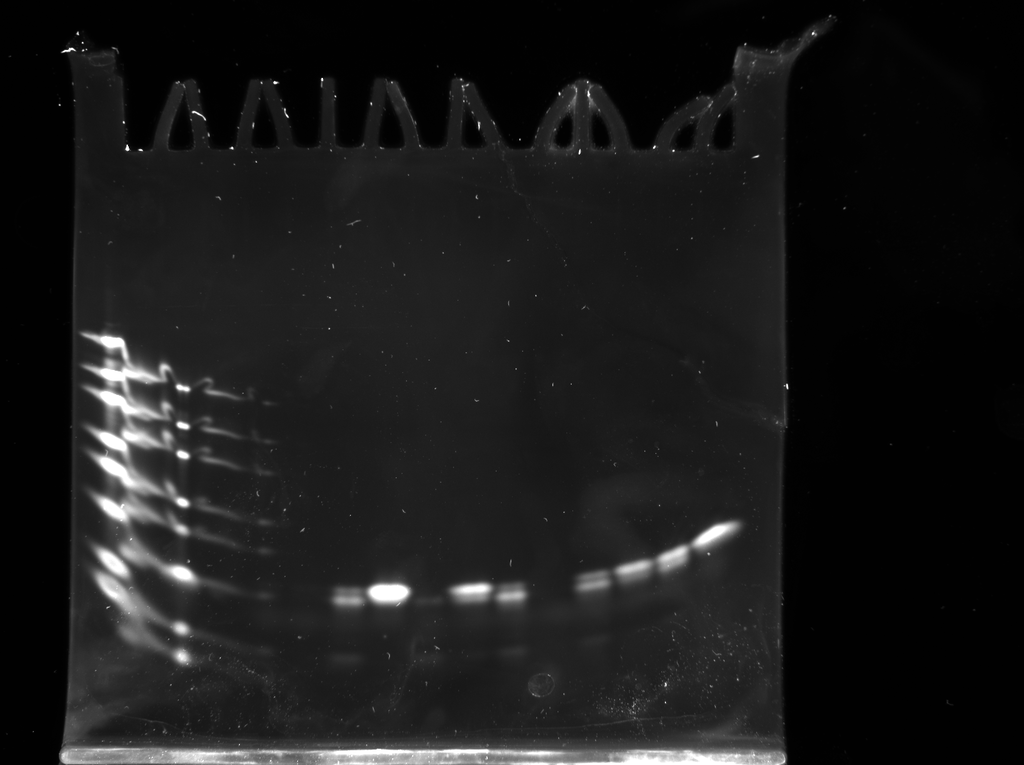
\includegraphics[width=6in]{./gel1.png}
\label{}
\caption{Gel 1}
\end{figure}

\begin{figure}[ht]
\centering
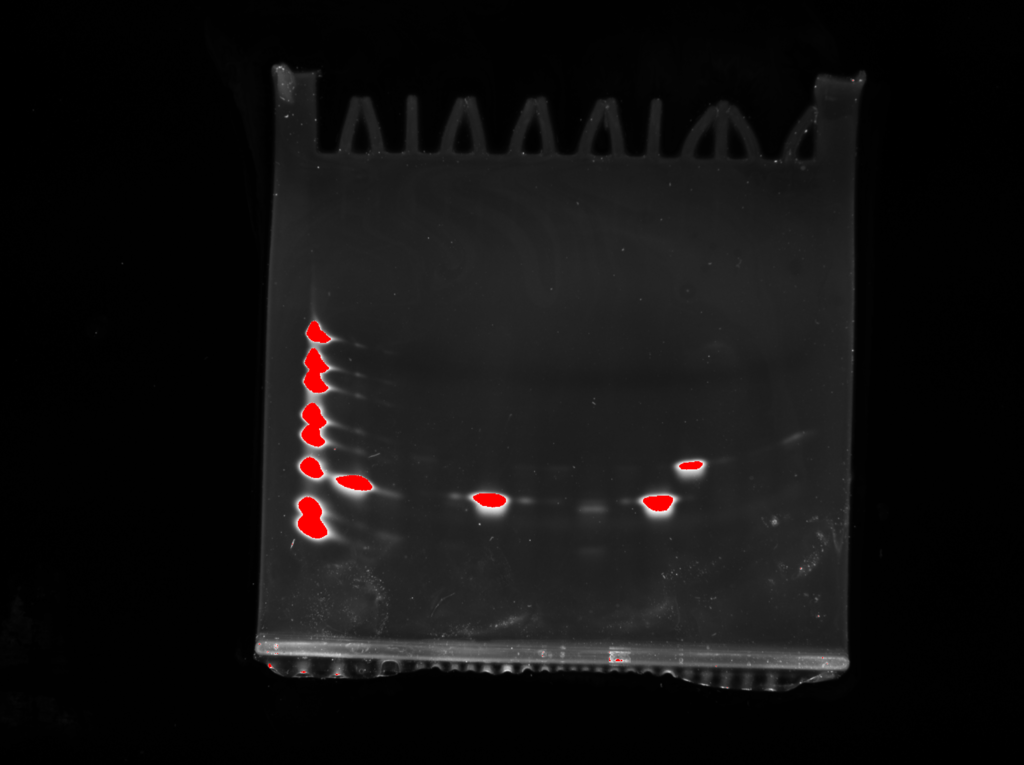
\includegraphics[width=6in]{./gel2.png}
\label{}
\caption{Gel 2}
\end{figure}

\bibliographystyle{ieeetr}
\bibliography{main}
\end{document}
